

\chapter{Úvod}
V úvode by som Vás rád krátko zoznámil s témou svojej bakalárskej práce, ktorá sa venuje téme Systému monitorovania stavu plánovacích úloh. Tento systém sa skladá z užívateľského rozhrania, ktoré je vytvorené prostredníctvom Java open-source technológií, ktoré bežia na javovskom serveri. Preto sa zameráme na všetky technológie, ktoré potrebujeme pre správne pochopenie a následnú implementáciu užívateľského rozhrania pre tento systém. Rovnako bližšie vysvetlím použitý open-source java server, ktorý je nevyhnutý pre beh aplikácie. Rovnako bude treba správne pochopiť celý plánovací open-source plánovací systém Optaplanner, pre ktoré je užívateľské rozhranie určené. Tento systém umožňuje spúšťať definované užívateľsky definované problémy, ktoré systém prostredníctvom správnych algoritmov naplánuje a dospeje k správnemu riešeniu vhľadom na dostupný čas a dostupné algoritmy. Rovnako sa budem venovať testovaniu a vyhodnoteniu užívateľského rozhrania z hľadiska intuitívnosti, jednoduchosti a splnenia všetkých formálnych požiadavok. Rovnako uvediem testy potrebné k overeniu správnej činnosti aplikácie a použitý framework. Toto téma bolo vybraté z dôvodu môjho osobného záujmu o open-source technológie,rovnako o možnosti ich využitia a veľmi ma zaujala možnosť verejná zdieľania projektu medzi open-source komunitov, ktorá mi môže poskytnúť spätnú vazu, resp. môže túto prácu využívať v praxi, čo cieľ, ktorý by som rád prostredníctvom tejto práce dosiahol.

Dopísať podľa vyhodnotnenie podľa testovania a dotazníka.




\chapter{Java Enterprise edition 6}
\section{Motivácia}
V posledných rokoch prevláda tendencia tvorby komplexných informačných systémov, ktoré spracovávajú veľké množstvo dát. Preto sa zvyšuje tlak na vývojárov na tvorbu prostriedkov, ktoré dokáže takéto systémy ľahko a rýchlo vytvárať. Jedným z takýchto prostriedkov je platforma Java Enterprise Edittion (Java EE ), ktorá použijeme vo verzii 6, ktorá nám postačuje pre implementáciu aplikácie. Java EE je platformou, ktorá rozširuje základné možnosti jazyka Java o enterprise technológie, ktoré umožňujú tvorbu komplexnejší systémov, ktoré bežia na rôznych aplikačných serveroch. Jazyk Java je open source, rovnako ako aj všetky poskytnuté technológie, preto som sa rozhodol využívať tento programovací jazyk. Platforma Java EE je ďalej tvorená špecifikáciami pre podporu webových technológí, webových aplikácií, podnikovej logiky a \ldots. Nám budú postačovať prvé 3 špefikácie tejto platformy, ktoré rozobereme v nasledujúcej časti spolu s technológiami, ktoré ich reprezentujú. Na základe Javy boli implementované boli implementované rôzne java EE kontajnery, ktoré sú potrebné pre správu a beh aplikácie. My sa zameriame na open-source riešenia z dôvodou šírenia projektu ako open-source. Ďalšou výhodou použitia tejto platformy je použitie anotácií, ktoré zjednodušujú implementáciu výslednej aplikácie a spôsobia konfiguráciu danej komponenty pri nasadzovaní a za behu. Rovnako je zdôraznení princíp POJO(Plain Old Java Objects)\cite{pojobook} a zjednodušenie tvorba balíkov. V poslednom rade musí spomenúť princíp \uv{Convetion over configuration}, ktorý minimalizuje počet konfigurácií pre daný projekt. V nasledujúcej časti rozoberiem všetky potrebné špecifikácie doplnené o rôzne frameworky, bez ktorých by sa vývojový cyklus aplikácie nezaobišiel.


\section{Špecifikácia platformy}
Java EE  predstavuje platformu určenú na vývoj webových a podnikových aplikácií\cite{fitWeb}. Tieto aplikácie sú viacvrstvové z dôvodu lepšej prenositeľnosti, nasaditeľnosti a modifikovateľnosti. Frontend, predstavujúci užívateľské rozhranie a logiku na jeho ovládanie, pozostáva z webových frameworkov, stredná vrsta poskytuje bezpečnosť a transakcie. Najnižšia vrstva poskytuje pripojenie k databázam. Java EE je platformou, ktorá poskytuje širokú škálu aplikačných programových rozhraní(API), ktoré zjednodušujú, zkracujú a znižujú komplexnosť vývoja a nasadenia výslednej aplikácie. Jej vývoj neustále napreduje a je spravovaný Java Comunnity process(JCP). Aplikácie pre platformu Java EE sú vyvíjané prostredníctvom API, ktoré táto plaforma poskytuje. Medzi tieto API patrí napríklad: Java Server Faces, Java Persistence API, Enterprise Java Bean, \ldots.  Behovým prostredím sú aplikačné servery, ktoré pozostávajú zo servletov, JavaServer Pages, EnterpriseJavaBeans a iných technológií, ktoré sa starajú o správu aplikácie a jej nasadenie. Keďže je Java označovaná ako multiplatformovaná musí poskytovať prostriedky, ktoré je možné nasadiť naprieč rôznymi aplikačnými serverami. Medzi takýto prostriedok patrí bezpečnosť, ktorá je v riešená pomocou prístupových pravidiel, ktoré sú interpretované za behu aplikácie.
 V ďalších kapitolách si rozoberieme aplikaný model jazyka, ktoré je veľmi dôležitý pre pochopenie princípu činnosti aplikácií vyvinutých touto platformou. V ďalšej kapitole rozobereme aplikačný model platformy Java EE.  


\section{Aplikačný model}
Java EE definuje aplikácie, ktoré sú viacvrstvové(multitier). Aplikačná logika je rozdelená medzi komponenty podľa ich funkcie\cite{Pravidla}. Jednotlivé komponenty sa následne rôzne inštalujú na rôzne zariadenia v závislosti, do ktorého stupňa patria(Keďže každý stupeň môže byť fyzicky na inom aplikačnom serveri). Jednotlivé stupňe sa skladajú z rôznych komponent, pričom stupne sú rozdelené nasledovne:
\begin{itemize}
\item Klientský stupeň sa skladá z klientských komponenent, ktoré bežia na klientskom počítači
\item Java EE server sa skladá z webových a podnikových komponent, ktoré bežia na Java EE serveri
\item Databázový server ktorý sa skladá z enterprise information system komponent
\end{itemize}

Typicky beží medzi klientskom a databázou častou viac-vláknový Java EE server, ktorý býva označovaný skratkou EIS. Viacstupňovérozloženie môžete názorne vidieť na obrázku č. \ref{model}.
\begin{figure}[htb]

\begin{center}

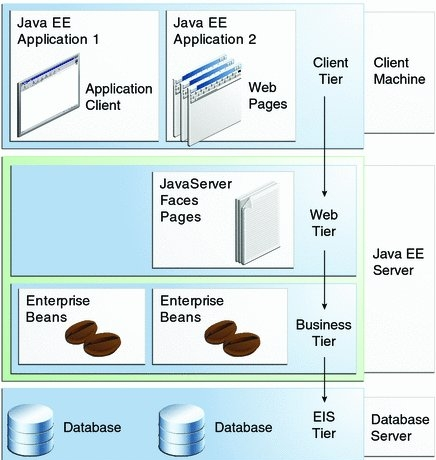
\includegraphics[scale=0.5]{model.jpg} 
\caption{Model Java EE [http://docs.oracle.com/javaee/6/tutorial/doc/]}
\label{model}

\end{center}

\end{figure}
Java EE aplikácia beží na klientskej stanici, býva obykle reprezentovaná tenkým klientom(webovým prehliadačom), nazývaným \uv{thin client}(pretože sa nedotazuje priamo na databázový server), alebo hrubým klientom, do ktoré je čiastočne vložená logika aplikácia. Klient môže byť reprezentovaný ako webový alebo aplikačný. Typický webový klient pritom pozostáva z:  Webové prehliadača, ktorý zobrazuje stránky a dynamických webových stránok pozostávajúceho  z rôzneho značkovaciehojazyka(HTML,XHTML), ktoré sú generované webovými komponentami. Zložitá logika je vykonávaná strednou vrstvou, pričom klient len posiela požiadavky na Java EE server a ten prípadne sa dotazuje databázové servera a následne predáva výsledok. Klient môže poskytovať aj bohatšie užívateľské rozhranie, ktorá býva vytvárané technológiou Swing alebo Abstract Window Toolkit\cite{guibook}, po prípade sa vyskytuje aj prístup prostredníctvom príkazového riadku. V strednej časti obrázku sa nachádza Java EE server, na ktorom môžu bežať rôzne technológie v závislosti od požiadavky výslednej aplikácie a možností daného servera.  Stredná vrstva sa ešte delí na webový stupeň, ktorý je prezentovaný technológiami JavaServer Faces a Pages. Druhá časť strednej vrstvy takzvaná podniková vrstva býva reprezentovaná technológiu EnterpriseJava Beans, ktoré vytvárajú logiku aplikácie. Java EE server môže by reprezentovaný, ešte okrem spomenutých technológií, rôznymi inými dostupnými technológiami, v závislosti od možnosti aplikačného servera, ktorý môže byť open-source (JBoss, Tomcat, GlassFish) alebo komerčný (IBM WebSphere,BEA WebLogic), ten obsahuje rôzne komponenty, ktoré so sebou rôzne komunikujú a interagujú na požiadavky klienta a na druhej strane komunikujú s databázovým systémom a starajú sa o beh aplikácie a jej nasadenie. Posledná časť predstavuje databázový server, ktorý obsahuju dáta, ktoré klient požaduje pri svojom požiadavku, tento server sa nazýva "EIS". Pre prístup k nemu sa používa buď nový prístup, ktorý sa nazýva objektovo-relačné mapovanie, ktoré využíva rozličné ovládače pre prístup k databázovému systému(napr. JBDC).

V nasledujúcej kapitole sa zameriame na technológie strednej vrstvy, ktoré sú nevyhnuté pre tvorbu a pochopenie činnosti navrhnutej aplikácie.


\section{Webové komponenty}
Java EE webové komponenty sú softwarové komponenty, ktoré spracovávajú prichádzajúci HTTP požiadok a poskytujú naň odpoveď. Všetky Java EE webové komponenty sú postavané na servletoch. ervlety sú javovské triedy , ktoré dynamicky spracovávajú požiadavky a tvoria odpovede.Súčasťou servletov alebo webových stránok, ktoré sú technológie JavaServer Faces technológiu(JSF) and JavaServer pages(JSP). Servlety podporujú automatickú správu sedenia, prostriedky pre vytváranie a ničenie servletov.  Technológie JavaServer Faces a JavaServer Pages podporujú spracovanie užívateľských vstupov a ich predanie a spracovanie podnikovou logikou. Pre implementáciu výslednej aplikáciu bola použitá JavaServer Faces technológia, ktorá poskytuje dostatočné možnosti pri tvorbe webových stránok. V rámci webových komponent spomeniem technológiu, ktorá je potrebná pre pochopenie funkčnosti aplikácie. Ide o technológiu Web Service.



\begin{figure}[htb]

\begin{center}

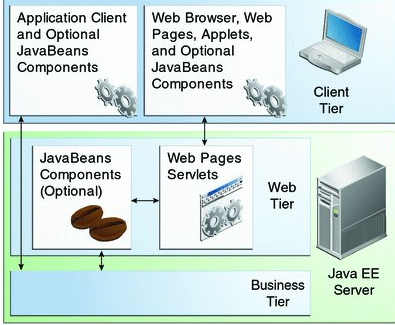
\includegraphics[scale=0.5]{webtechnology.jpg} 
\caption{Webové komponenty [http://docs.oracle.com/javaee/6/tutorial/doc/] }
\label{web}

\end{center}

\end{figure}
Na nasledujúcom obrázku č.\ref{web} je ukázaný princíp fungovania webových komponent. V hornej časti obrázku sa nachádza klientská vrstva, ktorá obsahuje buď len webový prehliadač po prípade Applety alebo JavaBean komponenty, ktoré čiastočne obsahujú logiku aplikácie. Na druhej strane môže byť klient reprezentoný aplikačným klientom, ktorý obsahuje obsahuje úplnú prezentačnú logiku aplikácie a teda v tom prípade, odpadá potreba spracovania vstupov po prípade nejaké generovania html stránky. Takýto klient komunikuje už len priamo s Java EE serverom, konkrétne podnikovým stupňom, ktorý implementuje zvyšnú logiku aplikácie a je reprezentovaný technológiou Enterprise Java Beans. V prípade, že máme k dispozícií tenkého klienta, klient komunikuje prostredníctvom webové prehliadača s HTML alebo XHTML stránky, ktoré sú vytvorené technológiou, ktoré spracovávajú požiadavok od klienta(vstupy) a následne komunikuje s podnikovým stupňom, ktorý obsahuje logiku reprezentovanú Enterprise Java Beans technológiou, ktorý následne môže komunikovať s databázovým serverom. Odpoveď je následne \uv{predaná} stránkám vytvorené prostredníctvom JavaServer Faces alebo JavaServer Pages technológiou a následne zobrazená užívatelovi v podobe výstupu na webovú stránku. V nasledujúcich dvoch podkapitolách sa bližšie pozreme na technológie JavaServer Faces a JavaServer Pages.


\subsection{JavaServer Faces}
JavaServer Faces(JSF)  je framework pre tvorbu užívateľských rozhraní webových aplikácií. Tento framework beží na Java EE serveri. Tento framework poskytuje sa skladá z ďalšieho frameworku, ktorý obsahuje rôzne komponty pre zobrazenie informácií, užívateľských vstupov, spracovanie udalostí, navigáciu medzi stránkami. JSF vytvára aplikácie na základe MVC - Model-View Controller. Aplikácia, ktorá je vytvára týmto frameworkom pozostáva z webových stránok, grafických komponent, sadou komponent naviazané na serverovú časť. Môže obsahovať rôzne desktriptory a konfiguračné súbory, ktoré nám pomáhujú pri nasadzovaní aplikácie. Základom JavaServer Faces je Facelets, čo je vlastne framework , ktorý slúži k tvorbe prezentačnej vrstvy webových aplikácií. Tento jazyk pomáha vytvárať JSF pohľady prostredníctvom HTML a buduje strom komponent. Facelets využíva XHTML pre vytváranie stránok, rovnako podporuje Facelets tag library, ktoré obsahujú obsahujú rôzne dekláracie komponenty, ktorých použitie je nevyhnuté pokiaľ chceme použiť nejakú komponenty z danej knižnice. Ttagy jednotlivých knižníc sú rozlišované na základe menných priestorov a to nasledovne: 
 
\begin{table}

  \begin{tabbing}
    Knižnica ~~~~\= URI ~~~~\= Zavedený prefix ~~~~ \= Popis ~~~~
    \= 34 \kill
    \bfseries Knižnica \>
    \bfseries URI \>
        \bfseries Zavedený prefix \>
    \bfseries Popis. \\[2mm]
   JSF Facelets Tag Library \> 	http://java.sun.com/jsf/facelets  \>	ui:  \>	Tagy pro tvorbu šablón \\
JSF HTML Tag Library  \>	http://java.sun.com/jsf/html  \>	h:  \>	Tagy komponent uživatelského rozhrania \\
JSF Core Tag Library  \>	http://java.sun.com/jsf/core  \>	f: 	 \> Tagy s funkcionalitou nezávislou na RenderKitu \\
JSTL Core Tag Library  \>	http://java.sun.com/jstl/core  \>	c:  \>	Tagy jadra JSTL – cykly, podmienky \ldots. \\
JSTL Functions Tag Library   \> http://java.sun.com/jstl/functions  \>	fn:  \>	Tagy JSTL pro funkcie  \\
    \end{tabbing}
\caption{Tagy knižníc [http://docs.oracle.com/javaee/6/tutorial/doc]}
\end{table}

Facelets stránky používajú XHTML 1 a CSS. Facelets od JSF 2.0 nahradzuje pôvodne používanú technológiu JavaServer Pages, ktorá sa pôvodne starala o tvorbu prezentačnej vrstvy aplikácií. Neoddeliteľnou súčasťou technológiu je Expression Language(EL), ktorý umožňuje dynamicky pristupovať k metódam javovských tried, rovnako dokáže získať a nastaviť hodnotu danej komponenty.Pri preklade sa vygenerejú z facelets a EL html komponenty, ktoré sú viazané na javovské triedy, ktoré sa nazývaju \uv{Managed Bean}. Managed Bean sú javovský trieda, ktoré zabezpečujú predávanie údajov medzi rôznymi podnikovými komponentami(tvorenými EnterpriseJava Bean technológiou) a webovou stránkou. Takáto trieda dokáže za behu spracovávať údaje zadané na webovú stránku, rovnako dokáže obstarať validáciu vstupov,  následne metódy a vlastnosti, ktoré sú volané alebo sú predávané údaje z vygenerovavnej stránky(HTML alebo XHTML) do managed bean-y alebo opačne. Aby bola v aplikácií \uv{známa} daná managed bean-a je potrebnú ju zaregistrovať v súbore faces-config.xml. Faces-config-xml je vlastne konfiguračný súbor, ktorý obsahuje zoznam managed bean a cestu k ním v rámci balíkovania, rovnako aj typ managed beany. Typ managed beany môže byť: 
\begin{itemize}
\item @RequestScoped Managed beana pokiaľ prežíva HTTP požiadavok. Vytvára sa pri vytvorený požiadavku a zaniká pri zrušení HTTP požiadavku
\item @NoneScoped Managed Beana existuje tak dlho ako existuje vyhodnotenie Facelets na stránky, po vyhodnotení zaniká
\item @ViewScoped Managed beana prežíva pokiaľ existuje interakcia s danou JSF stránkou. Vytvára sa pri žiadosti o danú stránku a zaniká pokiaľ užívateľ prejde na inú JSF stránku
\item @SessionScoped Managed bean prežíva tak dlho pokiaľ existuje HTTP sedenie. Vytvára sa pri 1.požiadavke o danú stránku a zaniká pri invalidácií daného HTTP sedenia
\item @ApplicationScoped Managed Bean prežíva dokiaľ existuje aplikácia. Je vytvorená pri prvej interakcii s aplikáciou a zaniká pri ukončení aplikácie
\item @CustomScoped Managed Bean existuje dokiaľ existuje záznam o bean-e v v custom Map, ktorá je vytvorená pre existenciu danej beany
\end{itemize}
Rovnako je možné v tomto konfiguračnom súbore nastaviť validačné triedy, reakcie na chyby a iné. Rovnako každá JSF aplikácia môže obsahovať konfiguračný súbor web.xml, ktorý je webový aplikačný deskriptov nasadenia. Tento súbor definuje všetky informácie, ko ktorých musí server vedieť, napr. použité servlety, inicializačné parametre, uvítacie stránky, \ldots.
\subsection{JavaServer Pages}
JavaServer Pages technológia je jazyk, ktorý umožňuje priamo vkladanie Java kódu do HTML kódu. Pre vloženia ohraničenie java kódu v HTML stránke sa používajú nasledujúce značky: <\% \%> medzi, ktoré sa vloží príslušný java kód. Takéto časti v html stránky sa nazývaju skriptlety. Tieto skriplety sú dynamické, to znamená, že sú vykonávané za behu aplikácie. Výhodou tejto technológie, že je napísaná v Java a tento jazyk je komplexnejší a bezpečnejší. Rovnako pri žiadosť o JSP stránku(html stránka s príponou JSP, ktorá obsahuje nejaký skriptlet) je, že pri zmene sa nemení celý obsah stránky ale len jej časť, ktorá bola zmenená. Takže takéto JSP stránky sú dynamické a umožňujú zmenu obsahu za behu.

\begin{figure}[htb]

\begin{center}

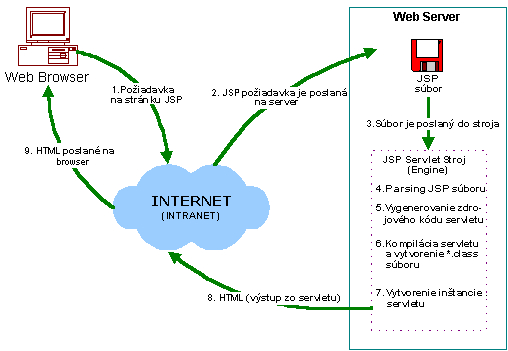
\includegraphics[scale=0.5]{architecture.jpg} 
\caption{JSP architektúra [http://interval.cz/clanky/javaserver-pages-pro-vsechny/] }
\label{jsp}

\end{center}

\end{figure}
Na nasledujjúcom obrázku č.\ref{jsp}
Užívateľ je reprezentovaný webový prehliadačom, ktorý zažiada o JSP stránku. Táto požiadavka je predaná Java EE serveru, ktorý zistí, že sa jedná o požiadavku na JPS stránku. Preto je požiadavok spracovaný JSP servlet strojom. Ten skontroluje početnosť požiadavok na danú stránku, pokiaľ ide o 1. tak stránku vygeneruje v opačnom prípade ju prekontroluje. Následne sa vygeneruje špeciálny servlet, ktorý ako základ použije JSP súbor. Kód tohto servletu je skompilovaný a je vytvorená jeho inštancia. Výstupotom zo servletu, ktorý vznikol ako požiadavka o JSP stránku je html stránka, ktorá je predaná užívateľovi, ktorý si ju zobrazí. V poslednom rade by som uviedol životný cyklus JavaServer Faces stránky, ktorý začína generovaním HTTP požiadavku klienta o stránky a končí odpoveďou servera stránkou, ktorá je preložená do HTML kódu.
Životný cyklus generovania odpovedi na strane servera je oveľa zložitejší, keďže sa berú do úvahy rôzne interakcie medzi komponentami na stránke a iné závislosti. Celý štandardný cyklus cyklus spracovania požiadavky a následne generovania odpovedi je popísaný na nasledujúcom obrázku.
\begin{figure}[htb]

\begin{center}

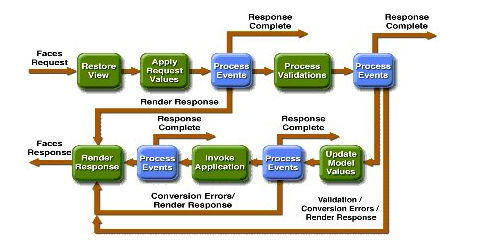
\includegraphics[scale=0.5]{jsflifecycle.jpg} 
\caption{JSF životný cyklus [http://docs.oracle.com/javaee/1.4/tutorial/doc/] }
\label{lifecycle}

\end{center}

\end{figure}

\subsection{Web Service}
Web Service  je sotwarový systém navrhnutý na podporu inteoperability medzi rôznymi zariadeniami prostredníctvom počítačovej siete. Komunikácia prebehia prostredníctvom HTTP protokolu vymenieňaním XML správ. Tieto aplikácie poskystujú interoperabilitu medzi rôznymi platformami naprieč počítačou sieťou. Web Service umožňuje komunikáciu medzi rôznymi aplikáciami, ktoré bežia na rôznych platformách, napr. Java aplikácie založené na Windowse komunikujú s Net, aplikáciami bežiaci na Linuxe. Tento aspekt je aspekt je umožnený tým, že aplikácie komunikujú prostredníctov HTTP protokolu. Na konceptuálnej úrovni môžme web service chápať ako softwarové komponenty poskytujúje prístup ku koncovému bodu. Týmto koncovým bodov môžme rozumieť systém inej organizácie, od ktorej potrebuje získať nejaké dáta. Rovnako sa môže jednať aj o systém v rámci organizácie. Komunikácia prostredníctvom web service sa delí na 2 učastníkov. Prvý účastník produkovateľ(producer), ktorý vytvára požiadavok a spotrebiteľ(consumer), ktorý prijíma požiadavok. Komunikácia prebieha medzi týmto dvoma učastníkmi výmenov správ. Web service môže byť technicky implementovaný rôznymi možnosťami a prostredníctvom Big Web Service alebo Restful WebService. Tento typ technológie bol zvolený z dôvodu potreby komunikácie užívateľského rozhrania so systémom na výpočet, ktorý sa nachadzá na inom výpočetom zariadení a tieto zariadenia si vymieňajú informáciu prostredníctvom HTTP protokolu. Umožňuje nám teda zdieľať funkčnosť kódu prostredníctvom siete a jej vzdialené volanie. Ďalšou výodou tejto technoógie využívajú štandardizované protokoly komunikájuce, čo umožňuje jednoduchú interoperability medzi inými systémami. Keďže táto technológia používa pre komunikáciu HTTP protokol využíva pre komunikuje prostredníctvom štandardnej počítačovej siete, čo žnižuje náklady na prevádzkovanie na rozdiel od iných proprietárnych technológií.

\subsubsection{"Big" Web Services}
Big Web Service je druh web service, ktorá pre svoju implementáciu používa API JAX-SW\cite{fitWeb} "Big" . Tento typ web service umožňuje vytvárať web service orientované na spráce alebo web service, ktoré využívajú vzdialené volanie procedúr(RPC). Tento typ web service využíva XML správy, spolu so Simple Object Acess Protocol(SOAP) a XML jazykom, ktorý definuje architekrúru a formát správ.
\begin{figure}[htb]

\begin{center}

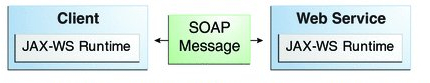
\includegraphics[scale=0.5]{webservice.jpg} 
\caption{Big Web Service [http://docs.oracle.com/javaee/6/tutorial/doc/] }
\label{com}

\end{center}

\end{figure}
Nasledujucí obrázok č. \ref{com} ukazuje spôsob komunikácie medzi klientom, ktorý sa nachádza v ľavej časti obrázku a web service, ktorá sa nachádza vpravej časti obrázku. Komunikácia prebieha prostredníctvom vymienania SOAP správ. Rovnako ako na klientovi tak aj web service obsahuje potrebné API, ktoré spracováva SOAP správy a predáva ich ďalej.


 Tento typ Web Service obsahuje definíciu pre Web Service vo formáte WSDL, ktorý je čitatelný aj počítačom vo formátet xml. Formát SOAP správ a definíciu jazyka WSDL rozhrania môže znížiť zložitosť vývoja aplikácií, webových služieb, pričom toto rozhranie je definované prostredníctvom XML. SOAP definuje štruktúru kódovania správ, konvenciu pre reprezentáciu web service, rovnako aj spôsob volania a odopovedi. Správy volania a odpovedí web service sú vymieňané prostredníctvom SOAP správ prostredníctvom HTTP protokolu. JAX-WS API je pomerne komplikované, preto celá komplexnosť je vývojarovi zakrytá a je jediné, čo definuje vývojár sú metódy, ktoré je možné vzdialene volať. Rovnako vývojár nespracováva SOAP správy, ale celá táto problematika je riešená prostredníctvom prostredníctvom API. Veľká výhoda je platformová nezávislosť, ktorá je dosiahnutá prostredníctvom Javy. Tak isto toto API umožňuje prístup k ne-Javovským web service, čo prináša veľkú flexibilitu. Čo sa týka vývoja web service, tak sa jedná o jednoduchú Java triedu, ktorá používa anotáciu javax.jws.WebService, konkrétne anotáciu @WebService, ktorá označuje, že sa jedná o web service endpoint. Táto trieda následne definuje metódy, ktoré môžu byť vzdialené volané. Aby moha byť metóda metódou web service musí byť anotovaná prostredníctvom anotácie  javax.jws.WebMethod @WebMethod. API ponuká aj ďalšie možnosť ako ovplyvňovať životný cyklus web service.




\section{Java Persistence API}
Java Persistence API(JPA) je špecifikácia jazyku Java, ktorá poskytuje prístup, spravovanie dát medzi Java objektmi a triedami a relačnými databázami. Základnou jednotkou JPA je entita, čo je vlastne odľahčený perzistentný doménový objekt, ktorý typicky reprezentuje tabuľku v relačnej databázy a každá jej inštancia je riadkom v  tabuľke. Základný artefaktom v programovaní je pre entity entitná trieda, ktorá obsahuje vlastnosti, ktoré priamo odpovedajú stĺpcov v databáze. Každá entitná trieda priamo musí byť anotovaná javax.persistence.Entity anotáciou. Rovnako musí mať parametrický konštruktor, aby bolo možné vytvárať nové entity. Každá vlastnosť musí pritom spĺňať princíp POJO(Plain Old Java Object), čo znamená, že pre každú metódu musí existovať metóda get a set. Jednotlivé hodnoty môžu byť priamo validované prostredníctvom API JavaBeans Validation prostredníctvom, ktoré je možné definovať anotácie avax.validation.constraints, ktoré obsahuje rôzne vlastnosti, ktoré musia vlastnosti spĺňať(nenulovosť, požiadavky na špeciálny formát vlastnosti, \ldots). Každá entitná trieda má unikátny identifikátor. Týmto identifikátor sa chápe primárny kľúč, ktorý môže byť, môže byť jednoduchý alebo môže byť zložený. Jednoduchý primárny kľúč sa v entitnej triede uvádza prostredníctvom anotácie javax.persistence.Id. V poslednom rade môže byť každá entitna vo vzťahu s inými entitami. Na označenej danej vlastnosti, že sa súčaštou vzťahu s nejakou entitou používame anotácie One-to-one, One-to-many, Many-to-one, Many-to-Many, pričom prostredníctvom anotácie javax.persistence.JoinColumn nám zabezpečuje naviazanie vzťahu s inou entitou. JPA ponúka aj iné, pokročilé možnosti mapovania, pre naše potreby nám budú stačiť nasledujúce vedomosti. Spravovanie entít je zabezpečované triedou EntityManager, ktorá je reprezentovaná triedou javax.persistence.EntityManager. Každá inštancia tejto triedy je spojená s perzistentný kontextom a určitou množinou entitný tried. Entity manager vytvára a odstraňuje perzistentne entity, umožňuje vyhľadávať entity, rovnako aj vytvárať SQL dotazy nad databázou. Entity manager pracuje s persistencu unit, čo odpovedá definíci entitných tried, s ktorými entity manager pracuje, teda definuje databázové tabuľky, s ktorými entity manager pracuje. Persistence unit sú definované v súbore persistence.xml. JAP rovnako definuje vlastný jazyk Java Persistence Query Language(JPQL), čo je jazyk podobný jazyku SQL, ktorý využíva trieda EntityManager pri svojej práci. Je to jednoduchý reťazcovo založený jazyk na spravovanie entít a vzťahou. Výhodou je, že tento jazyk je nezávislý na zvolenej databázovej technológií a má objektové vlastnosti, teda pri dotazoch nepoužívame konkrétne názvy tabuliek ale názvy entitný tried a jej vlastností. Problém JPQL je typová nebezpečnosť, čo vyžaduje pretypovanie výsledkov dotazu z entity manager-a. To môže spôsobiť chyby, ktoré nemusia byť odchytené počas kompilácie. JPA definuje ešte Criteria API, ktoré je využívané k vytváraniu dotazovou nad entitami a vzťahy, ktoré sú typovo bezpečné. Výhodou tohto API, pre použitie na dotazovanie, je rovnako možnosť vytvárať dynamické dotazy, ktoré majú lepšiu výkonnosť ako JPQL. Pre naše potreby budemé používať obe varianty dotazovania nad dátami v databazy. V poslednom rade treba spomenúť, že JPA je nezávislé nad použitou databázou technológiou, je možné vytvárať dotazy nad MySQL, SQL databázou \ldots. Nakoniec treba zdôrazniť, že JPA nie je konkrétna implementácia ale špecifikácie, implementácie JPA môže byť: Hibernate, TopLink, OpenJPA.


\section{Enterprise JavaBeans}
EnterpriseJavaBeans(EJB) je technológia, ktrorá vytvára Enterprise Beans(EB), ktoré predstavuju Java EE komponenty.EJB ďalej predstavuje spravovateľnú, server-side, komponentnú architektúru pre modulárne konštruovanie enterprise aplikácií. EB je server-side komponentov, teda beží v Java EE kontajneri. Podstatnou úlohou tejto komponenty je zapuzdrenie podnikovej logiky aplikácie. EB programátorov pri riešení častou opakovaných problémov, napríklad perzistencia, bezpečnosť \ldots. V prípade škálovatelnej aplikácie ponúka EB možnosť behu na viacerý zariadenia, rovnako pre väčší počet užívateľov môže existovať viacero EB, ktoré môžu byť rozlične veľké a mať rozličné inštancia v závislosti od požiadavky klienta. EB sa môžu rôzne nachádzať na zariadeniach, ktoré sú prepojené prostredníctvom počítačovej siete a môžu byť volané prostredníctvom štandardného klient/server modelu. Také aplikácie môže byť distribuované a teda poskytovať obsluhu veľkého množstva užívateľov.


EB sa delia na 2 kategórie:
\begin{itemize}
\item Message-driven - Vykoná úloha pre klienta; voliteľne môže implementovať webové služby
\item Session - Pôsobí ako poslucháča pre určitý typ správ, ako je API Java Message Service

\end{itemize}


\subsection{Session Bean}
Session bean je typ EB, ktorá zapúzdruje podnikovú logiku, ktorá môže byť vyvolaná lokálne, vzdialene alebo prostredníctvom web service klienta. Prístup k session bean sa dejé prostredníctvom volania metód bean-y. Bean-a následne vykoná podnikový kód na serverovej strane. Takýto typ beany nie je perzistentný. Táto beana môže byť ešte 3 typov:
\begin{itemize}
\item Stateful Session Bean - beany udržuje hodnoty premených, každá beana reprezentuje unikátny stav klienta/bean sedenia. Stav komunikácie beany a klienta sa často nazýva \uv{conversational state}, môže mať len 1 klienta, rovnako sedenie môže interagovať len s 1 klientom. Stav je zachovávaný počas klientského/bean sedenia. Pokiaľ sa sedenie odstrániť stav zminzne.
\item Stateless Session Bean - Neudržuje conversational state s klientom. Počas invokácie metódy takejto beany môže inštancia obsahovať premenné, ktoré môžu obsahovať špecifický stav vzhľadom na klienta, alebo len po počas invokácie metódy. Stav beany špecifický pre klienta nepretrváva, ale tento stav môže pretrvať v poll stateless bean počas ďalšej invokáciu metódy. Rovnako jednotlivé inštancie stateless bean sú ekvivalentné takže môžu byť priradené ľúbovoľnému klientovi. Z toho vyplýva, že podporuje viacnásobný prístup klientov a lepšiu škálovatelnosť. Tento typ session beany môže implementovať web service.
\item Singleton Session Bean - Tneto typ beany je inštanciovaný len raz a pretrváva počass celého životného cyklu aplikácie. Využíva sa pri zdieľaní a súčasnom prístupe viacerých užívateľov. Rovnako aj tento typ session beany môže implementovať web service, rovnako udržuje stav medzi invokáciami metód klienta. Tento typ beany môže byť využitý pre špecifické akcie aplikácie, napr. ukončenie aplikácie, štart aplikácie, \ldots, pretože pretrváva počas celého životného cyklu aplikácie.
\end{itemize}

Tento typ beany môžme použiť pokiaľ potrebuje udržať stav medzi klientskými volaniami metód, rovnako pokiaľ potrebuje odľahčiť aplikáciu a zvýšiť výkonnosť použijeme tento typ beany konkrétne stateless session bean. Tieto beany dokážu implementovať web service.

\subsection{Message-driven Bean}
Message-driven bean je typ EB, ktorá umožňuje Java EE aplikáciám asynchronné spracovanie správ. Tento typ beany sa správa rovnako ako Java Message Service(JMSS)\cite{messagebook} naslúchať správ, ale narozdiel od JMS beana prijíma JMS správy. Tieto správy môžu byť poslané rôznymi Java EE komponentami, alebo JMS aplikáciou alebo aj iným systémom, ktorý nepoužíva Java technológiu. Tieto beany nespracovávajú len JMS správy ale aj iné typy správ. Zásadny rozdiel je medzi message-driven bean a session bean v zásade v tom, že sa k takému to typu beanu nepristupuje prostredníctvom rozhrania a invokácie metód. Tento typ beany obsahuje len bean triedy. Message-driven bean neudržuje dáta alebo conversational state pre klienta. Všetky inštancie takého typu beany sú ekvivalentné, to umožňuje EJB kontaineru priraďovať správy ľubovoľne message-drive bean inštancii. Jedna inštancia beany môže spracováva rozličné správy od klientov. Inštancia premenných môže udržovať stav spracovania klientských správ napr. JMS API connection, databázové pripojenie, \ldots. Klienti pristupujú k message-driven bean, napr. zasielaní správ do cieľa pre message-driven beanu je MessageListener. Message-driven bean má ďalšie zaujímavé vlastnosti a to, že môžu byť vyvolané asychronne, žijú relatívne krátko a sú bezstavové. Pokiaľ správa dorazí do message-driven bean kontajner zavolá metódu onMessage, ktorá pretypuje JMS správy na jeden typ správy a naloží s ňou podľa podnikovej logiky.  Výhodou tejto beany je posielanie asychrónnych správ, ktoré nevyťažujú tak prostriedky servera.



\section{Convetion over Configuration}
Convetion over Configuration je sotwarový design, ktoré znižuje počet rozhodnutí, ktoré musí urobiť vývojár a zároveň zvyšuje jednoduchnosť, ale nie na úkor flexibility. Po zjednodušení môže tento princíp chápať v zmysle, že vývojár nakonfiguruje len \uv{nezvyklé} aspekty aplikácie. Tento princíp sa snaží odstrániť množstvo konfiguračných súbor, ktoré robia daný projekt neprenositeľný.
Jedným z prostriedkom, ktorý implementuje daný princíp je Maven. Maven je stavebný automatizačný nástroj, ktorý je primárne používaný pre Java projekty. Maven definuje spôsob ako bude sotware zostavený, rovnako aj definuje závislosti(Depency Management). Celý obsah je definovaný v XML súbore, v ktorom sa rovnako definujú závislosti na externé moduly, poradie zostavovania komponent a požadované pluginy. Obsahuje predefinované úlohy ako kompilácia, testovanie, balíkovanie a nasadzovanie. Maven dynimacky sťahuje Javovské knižnice a maven pluginy z jedného alebo viacerých repozitárov ako napr. Maven 2 Central Repository a ukladá ich v lookálnej cache. Maven projekty sú konfigurované prostredníctvom xml súbor, ktorý využíva Project Objec Model a nazýva sa pom.xml, pričom sa nachádza v koreňovom adresári projektu. Nasledujúci obrázok ukazuje štandardnú adresárovú štruktúru maven projektu:

\begin{figure}[htb]

\begin{center}

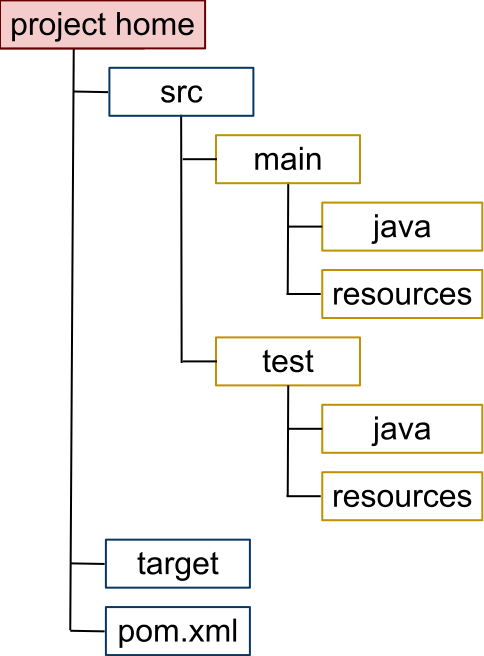
\includegraphics[scale=0.5]{maven.jpg} 
\caption{Maven adresárová štruktúra [http://maven.apache.org/] }
\label{maven}

\end{center}

\end{figure}
obrázok č. \ref{maven} ukazuje základnú adresárovú štruktúru maven projektu. Každý maven projekty sa skladá z project home, ktorý obsahuje súbor pom.xm a všetky ostatné podadresáre. Ďalej sa skladá z priečinkkov src, kde sa nachádzajú zdrojové kódy a target, kde sa ukladajú preložené triedy\cite{mavenbook}. Adresár src sa ďalej skladá z adresáru main, ktorý ešte obsahuje adresára java, ktorý obsahuje java zdrojový kód pre daný projekt a resources, ktorý obsahuje prostriedky pre daný projekt ako sú rôzne súbore, ktoré obsahujú nastavenie prostriedkov pre daný projekt. Podadresár src sa skladá z adresára test, ktorý rovnako ako src obsahuje podadresár java, korom je umiestnený java zdrojový kód pre testovanie projektu. Podadresár test obsahuje ďalší adresár resources, ktorý obsahuje prostriedky potrebné pre testovanie. Celá táto štruktúra predstavuje základne adresáru štruktúru pre maven projekt a tak to robí viac prenositeľný. Jednotlivé závislosti pre projekt jednoducho definuje v súbore pom.xml. Preložením projektu sa preložia všetky triedy a uloźia do adresára tagert. Celý projekt môže byť pre väčsiu modularitu rozdelený na moduly, pričom každý modul rovnako splňuje základnú Maven adresárovú štruktúru. Každý maven projekt je možné dať ako cieľ jednú z fázy životného cyklu. Životný cyklus môže byť z jednej fáz: 1. validate - validácia korektnosti projektu a kontrola dostupnosti potrebných informácií pre projekt ,2.kompilácia - kompilácia zdrojového kódu projektu, 3.test - testovanie zkompilovaného zdrojového kódu, táto fáza nie je vyžadovaná 4.package - zabalenie zkompilovaného projektu do balíku, napríklad jar, 4. integration-test - spracovanie a nasadenie balíku pokiaľ je to potrebné do prostredia, kde môžu bežať integračné testy, 5.verify-run - beh a overenie balíku, že spĺňa všetky kritéria pre spustenie, 6. install - inštalácia balíku do lokálneho repozitára, v prípade, že potrebuje použiť balík ako závisloť 8.deploy - nasadenie projektu do kontejneru a spustenie.
Jednotlivé fázy môže spustiť príkazom \uv{mvn názov životného cyklu}, napríklad mvn package. Na porovanie výhod Maven som použil nástroj Apache Ant. Ant nástroj nedefinuje presnú adresárovú štruktúru a podporované úlohy narozdiel od maven-u. Definovanie úloh Ant-u sa môžu nachádzať vo viacerých súboroch, pričom každý súbor môže definovať jednu úlohu. Výhodou Ant-u je optimalizácie XML jazyka pre potreby Ant-u pre jasnu definíciu, čo robí a od čoho závisí. Laik je schopný okamžite pochopiť, čo vykonáva xml súbor ant-u.Na druhej strane výhodou Maven-u je, že vývojár, ktorý má skúsenosti s maven-om pochopí okamžite pri neznámom projekte štruktúru projektu a je schopný spustiť štandarné úlohy maven a pozná očakávaný výstup. Z tohto dôvodu som sa pochopil využiť Maven pre svoj projekt, ktorý má rovnako výhodu použítým Depency Management.


\section{Testovanie}
V poslednom rade musí technológie, ktoré budem používať pre testovanie. Základom testovania sú 2 technológie, ktoré sme použili jednouchou z nich je technológia JUnit a druhá z nich je technológia Arqullian.
V prvom rade by som sa rád venoval technológií JUnit. JUnit je unit testovací framework pre programovací jazyk Java. JUnit sa používa pre typ testovania, ktorý sa nazýva test-driven development a je jedným z kolekcie unit testovacích frameworkov. JUnit je linkovaný ako jar súbor pri kompilácií a býva súčaštou balíku org.junit. \cite{junitbook}. JUnit testovací inventár je javovský objekt. Testovacie metódy sú anotované prostredníctvom @Test anotácie. JUnit rovnako umožňuje vykonať kód pred spustením testu, to docielime anotovaním metód @Before anotáciou alebo po sputení testu, to docielime anotáciou @After. V testovacej metóde potom vykonáme nejaké kód a očakávaný výstup porovnáme s nami očakávaným výsledok prostredníctvom Assert. JUnit testy sú písané pre otestovanie konkrétnej funkčnosti kódu. Cieľom testovania prostredníctvom JUnit sú malé kúsky kódu, ako metódy alebo triedy. JUnit testy môže použiť rovnako pri písaní kódu alebo pri refaktorizácií na overenie požadovanej funkčnosti kódu. Všetky tieto výhody som využil pri testovaním malých kúskov kódu, ktoré vykonávali požadovanú fukčnosť.

Nakoniec by som rád spomenul technológiu Arquallian. Arquallian je testovací framework, ktorý vykonáva testy vo vnútri vzdialeného alebo vstavaného kontajneru alebo nasadí archív na kontajner, tak aby test mohol interagovať so vzdialeným klientom. Arquallian integruje aj ďalšie testovacie frameworky, napr. JUnit 4, TestNG 5, \ldots, rovnako aj iné frameworky Ant, Maven a iné. Musí zdôrazniť, že narozdiel od JUnit testov umožňuje testovanie v java EE kontajnery(GlassFish, JBoss)\cite{arqbook}. Tento framework má zásadnú výhodu na prenositeľnosť testov na rôzne podporované kotajnery. Testy môžu byť spustené rovnako z IDE tak aj zostavovacím nástrojom. Framework rozširuje aleb integruje existujúce testovacie frameworky. Framework automaticky zabalí do testovacej platformy všetky potrebné prostriedky. V poslednom rade treba spomenúť, že spustenie arquallian testu je veľmi jednoduché. Použitie arquallianu je dané použitím anotácie @RunWith Arquillian, ktoré zabezpeči spustenie testov po spustení. Následne arquallian sputí kontajner nasadí testovací archív, ktorý je daný anotáciou @Deployment. Archív obsahuje testy so špecickými triedami a knižnice. Testy sa následne vykonajú vo vnútri kotajneru. Čo znamená, že sa použijú všetky dependency a resource inject do testov, takže môžme pristupovať k EJB, rovnako môže pristupovať k databáze, \ldots. Na prvý pohľad vyzeráju arquallian testy ako štandardné JUnit testy. Arquallian umožňuej testovať reálne komponenty, ktoré interagujú s java ee kontajnerom. Arquallian umožňuje spustiť testy vo viacerých módov. Jedným z nich je mód In-cotainer, kde testovanie prebieha priamo v java ee kontajnery pre interakciu s java ee komponentami, druhá možnosť je Client mode, kde testovanie prebieha u klienta u ukazuje ako klient využíva aplikáciu, posledna možnosť je použiť Mixed mode, ktorý kombinuje obe predchádzajúce možnosti. V poslednom rade je potrebné nastaviť kontajner, ktorý sa použije na testovanie. Konfigurácia sa deje prostredníctvom xml súboru arquillian.xml.


\chapter{JBoss Aplication Server}
Aplikačný server(AS) je sotware, ktorý poskytuje vrstvu medzi operačným systémom a java ee aplikáciami. AS poskytuje základnú funkciu programom(prístup k súborovému systému, posielanie správ, \ldots), konkrétne enterprise aplikáciám. Vytvára vrstvu, ktorá zjednodušuje vývoj enterprise aplikácie. Dôvod použitia pre enterprise aplikácie je ten, že tieto aplikácie sú robustné a komplexné a spracovávajú súčasne veľké množstvo požiadavkou od klientov, pričom typickou aplikáciou môže byť webová aplikácia. Pomerne veľká skupina AS je vyvíjaná v jazyku Java. Dôvodom pre tento jazyk existencia štandardu pre enterprise aplikácie a to je Java EE. Nás bude zaujímať implementácia Java EE, ktorá sa nazýva JBoss AS.

JBoss, čo je vlastne skratka pre JavaBeans Open Source Applicatom Server, je aplikačný server, ktorý je založený na platforme Java a Java Enterprise Edition.\cite{jbossbook}. Tento typ AS je open-source, preto je možné jeho stiahnutie spolu so zdrojovými kódmi. Používanie aplikačného servera JBoss je veľmi jednoduché jeho spustenie môžte vykonať ručne prostredníctvom konzole a nájdeným inštalačného adresára JBoss-u a následne adresára bin, ktorý obsahuje skript run.sh, ktorý spustí AS. Druhou možnoštou je spustenie prostredníctvom IDE. Po spustení serveru je možné k nemu implicitne pristupovať na localhost na porte 8080 počítača. Základným stavebným kameňom JBoss AS je JBoss Microcontainer. JBoss Microcontaijner je refaktorizácia JBoss JMX Microkernel aby podporoval POJO nasadzovanie a samostatné použitie mimo aplikačného servera. Microcontainer plní funkciu jadra, do ktorého sa registrujú všetky služby. Služby, ktoré majú by prístupné sa registrujú v podobe managed beans. Microcontainer spravuje a riadi beh týchto služieb. Do AS sa registruje všetko jeho funkcionalita, vrátane Java Management Extention, ktorý umožňuje správu zaregistrovaný služieb. Prostredníctvom tohto rozhranie môžme spravovať všetky zaregistrované služby. JBoss implicitne podporuje databázový server Hypersonic SQL, ktorý má ale obmedzené možnosti, ktorý je určený len na testovanie. Do tohto databázove servera si služby ukladajú informácie.
Tento server je licensovaný pod GNU Lesser General Public License(GNU PL). Dôvod výberu tohto aplikačného servera je integrácia open-source technológií, ktoré sú založené na Jave. Rovnako ako JBoss poskytuje implementáciu širšej škály Java EE technológií, ktoré potrebuje pre vývoj svojej práce. Aplikácie, ktoré bežia na JBoss sú oveľa komplexnejšie.



V ďalšej časti sa zameriame na OptaPlanner, čo je vlastne na plánovací framework Optaplanne, pre ktorý je rozhranie navrhované.




\chapter{OptaPlanner}
OptaPlanner je odľahčený open source software a ďalšie prokračovanie frameworku JBoss Drools, ktorý optimalizuje plánovacie problémy.\cite{optaweb} Tieto plánovacie problémy môžu byť nasledujúceho charakteru: 
\begin{itemize}
\item Plánovanie agendy: plánovanie schôdzok, vymenovanie, práca údržby
\item Plánovanie vzdelávania: plánovanie lekcie, kurzov
\end{itemize}
\begin{figure}[htb]

\begin{center}

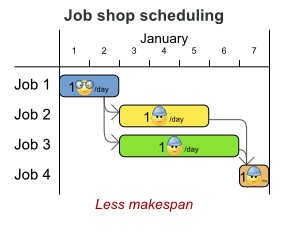
\includegraphics[scale=0.5]{fig/useCaseOverview.jpg} 
\caption{Job, Shop scheluding, prevzaté z http://www.optaplanner.org/ }
\label{obrazokUseCase}

\end{center}

\end{figure}
Obrázok č. \ref{obrazokUseCase} zobrazuje typické použitie OptaPlanner-u. Môžme vidieť v nasledujúcom obrázku vystupú 4 osoby, ktoré vykonávajú nejakú činnosť. Ich činnosť je špecifická a silne závisí od práce predchádzajúcich. Optaplanner sa snaží ich činnosti maximálne optimalizovať a jednotlivé činnosti zvoliť v následnosti tak, aby výsledná práca bola spravená za najkratší možný čas vzhľadom na činnosť, ktorá sa optimalizuje.


\subsection{NP-úplný problém}
Každý plánovací problém je NP-úplný problém.\cite{npbook} NP-úplné problémy sú nedeterministicky polynomiálne problémny, ktoré nie sú riešitelné v dostupnom čase, pretože sa nepodarilo nájsť deterministický algoritmus. Príkladom NP úloh môžme považovať: problém obchodné cestujúceho, \ldots .

Riešenia poskytnutým týmto frameworkom, ktorý využíva pokročilé optimalizačné algoritmy, sú dosiahnuteľné v reálnom čase. Dosiahnutie v reálnom čase znamená nájdenie 1 alebo viacerých riešení, alebo nenájdenie žiadneho riešenia vzhľadom na poskytnutý čas a optimalizačné algoritmy, ktoré sú implementované.

Každý plánovací problém je definovaný na základe obmedzení, ktoré musia minimálne spĺnať: \cite{optabook}
\begin{itemize}
\item Negatívne "hard" obmedzenie, ktoré nesmie byť porušené
\item Negatívne "soft" obmedzenie, ktoré by nemali byť porušené pokiaľ sa dá tomu vyhnúť.
\end{itemize}

Niektoré problémy môžu obsahovať aj pozitívne podmienky alebo odmeny, ktoré by mali byť splnené pokiaľ je možné ich splniť.

Tieto podmienky definujú skóre plánovacieho problému. Tieto podmienky môžu byť zapísané v Jave alebo v Drools pravidlách, ktoré značne zjednodušujú kód.

 Vytvorenie je pomocou pravidiel  môže robiť  oveľa jednoduchšie spájať mnoho pravidiel s mnohými akciami. Tieto pravidlá bývajú typicky definované pomocou XML súboru.

OptaPlanner pomáha  programátori riešiť obmedzenie problémov spokojnosti efektívne. Pod kapotou sa kombinuje optimalizačné heuristiky na výpočet skóre.



\subsection{Výsledky plánovacieho problému}

Tieto obmedzenia definujú výpočetné skóre problému plánovania. Každé riešenie problému plánovanie môže byť odstupňovaná so skóre. 

Plánovanie problému má niekoľko riešení. Existuje niekoľko kategórií riešení:
\begin{itemize}
\item Možným riešením je nejaké riešenie, či je alebo nie je ľubovoľný počet obmedzení. Problémy plánovanie mávajú neuveriteľne veľké množstvo možných riešení. Mnoho z týchto riešení sú bezcenné.
\item Uskutočniteľným riešením je riešenie, ktoré neporušuje žiadne (negatívne) tvrdé obmedzenia. Niekedy nie sú realizovateľné riešenie. Každý uskutočniteľné riešenie je možné riešenie.

\item Optimálnym riešením je riešenie s najvyšším počtom bodov. Problémy plánovanie mávajú jedno alebo niekoľko optimálnych riešení. K dispozícii je vždy aspoň 1 optimálnym riešením, a to aj v prípade , že neexistujú žiadne uskutočniteľné riešenie, a optimálne riešenie nie je možné .
\item Najlepším riešením je nájsť riešenie s najvyšším skóre zistené implementáciou v danom čase.

\end{itemize}

OptaPlanner podporuje niekoľko optimalizačných algoritmov ako efektívne prehrýzť týmto neuveriteľne veľkým množstvom možných riešení. V závislosti na prípade použitia, niektoré optimalizačné algoritmy dosahujú lepšie výsledky ako ostatné, ale to je nemožné povedať dopredu. Pri plánovaní , je ľahké prepnúť algoritmus optimalizácie, zmenou konfigurácie Solver na niekoľkých riadkov XML alebo kódu.


\newpage
\subsection{Ukážka XML configuračného súboru}
V nasledujúcom obrázku by som rád ukázal príklad XML configuračného súboru pre OptaPlanner.
 \lstset{
    language=xml,
    tabsize=3,
    %frame=lines,
    caption=Test,
    label=code:sample,
    frame=shadowbox,
    rulesepcolor=\color{gray},
    xleftmargin=20pt,
    framexleftmargin=15pt,
    keywordstyle=\color{blue}\bf,
    commentstyle=\color{OliveGreen},
    stringstyle=\color{red},
    numbers=left,
    numberstyle=\tiny,
    numbersep=5pt,
    breaklines=true,
    showstringspaces=false,
    basicstyle=\footnotesize,
    emph={food,name,price},emphstyle={\color{magenta}}}
    \lstinputlisting{cloudBalancingSolverConfig.xml}

\newpage
Konfigurácie solveru pozostáva z 3 častí: 
\begin{itemize}
\item Domail model configuration: Musíme Optaplanneru uviesť hlávnú triedu.
\item Configurácia skóre, ktorá hovorí Optaplanneru ako ma optimalizovať premenné. Pokiaľ používame hard a soft obmedzenia, použijeme "HardSoftScore". Musíme tiež uviesť ako vypočítať také skóre, v závislosti na našich požiadavkách. Ďalej sa, sme musíme  pozrieť do 2 alternatívy pre výpočet skóre: pomocou jednoduchej implementácie Java, alebo pomocou Drols DRL.Optaplanner bude hľadať riešenie s najvyšším skóre. Budeme používať HardSoftScore, čo znamená, plánovač bude hľadať riešenie s žiadnymi tvrdými obmedzeniami členenie (spĺňajú požiadavky na hardvér) a pokiaľ možno čo najmenej mäkkých obmedzenia členenie (minimalizovať náklady na údržbu).
\item Konfigurácia optimalizačných algoritmov

\end{itemize}

\subsection{Optimalizačné algoritmy}
V nasledujúcej časti textu si ukážeme optimalizačné algoritmy, ktoré používa optaplanner.
\begin{itemize}
\item First FIT - To je veľmi jednoduché greedy algoritmus aproximácie. Algoritmus spracováva položky v ľubovoľnom poradí. Pre každú položku, pokúsi sa umiestniť na položku v prvej priehradke, ktorý sa môže ubytovať položku. Ak nie je nájdený žiadna priehradka, otvára novú priehradku a kladie položku v rámci nového zásobníka.

\item Firt FIT Decreasing
\item Firt FIT Decreasing + heurestic local search

\begin{itemize}
\item Hill Climbing - hill climbing je matematická optimalizácia technika, ktorá patrí do rodiny miestneho vyhľadávania. Jedná sa o iteratívny algoritmus, ktorý začína s ľubovoľným riešenie problému, potom sa pokúsi nájsť lepšie riešenie tým, že postupne mení jeden prvok riešenia. Ak zmena vytvára lepšie riešenie zmeny sa opakujú až žiadne ďalšie zlepšenie nie je možno nájsť.\cite{algobook}




\item Tabu Search - Tabu search používa miestny alebo susedcký postup vyhľadávanie, tak že iteratívne presuvá z jedného možného riešenia x k lepšiemu riešeniu x  v susedstve x, kým sa niektoré kritérium zastavenia splní. Miestne postupy vyhľadávania sa často uviaznu v zle bodovaných oblastiach. V snahe vyhnúť sa týmto nástrahám a preskúmať oblasti hľadaného miesta, ktoré by mali zostať bez prehliadky inými miestnymi postupmi vyhľadávania, tabu search starostlivo skúma okolí každého toku ako hľadanie postupuje. Riešenie prijatí do novej štvrti  sú určené pomocou pamäťových štruktúr.

\item Simulated Annealing - Simulované žíhanie je všeobecný algoritmus pre globálne optimalizačné problémy lokalizovať dobré priblíženie k globálnej optimálnej danej funkcie vo veľkom vyhľadávacieho priestoru. To sa často používa pri hľadaní priestorov diskrétnych (napr. všetky výlety, ktoré navštevujú danú množinu miest). U niektorých problémov, môže simulované žíhanie byť účinnejšie ako vyčerpávajúci zoznam - za predpokladu, že cieľom je iba nájsť prijateľne dobré riešenie v stanovenú dobu, skôr ako tým najlepším možným riešením .

\end{itemize}

\end{itemize}


V ďalšej kapitole by som rád uviedol problematiku užívateľského rozhrania.
\chapter{Grafické užívateľské rozhranie}
V tejto kapitole sa zameráme na problematiku užívateľského rozhrania, ktoré vlastne je reprezentované prostredíctvom technológie Java Server Faces v kombinácií frameworkov Rich Faces a Twitter Bootstrap-u. Toto rozhranie bude umožňovať nahrávať pravidlá, zobrazovať výsledky, spúšťať, pozastovať a zobrazovať detaily úloh. Keďže táto výsledná aplikácia by mala byť použíteľná aj na mobilnom telefóne bol vybratý štýlovací framework Twitter Bootstrap, ktorý značne uľahčenie tvorbu takéhoto rozhrania.

\section{Twitter Bootstrap}
Twitter Bootstrapje veľmi jednoduchý a voľne dostupný súbor nástrojov pre vytváranie moderného webu a webových aplikácií.\cite{boot} Ponúka podporu najrôznejších webových technológií HTML , CSS , JavaScript a mnoho prvkov , ktoré je možné ľahko implementovať do svojej stránky. Pre použitie Twitter Bootstrap sú nutné základné znalosti HTML a CSS. Interaktívne prvky ako sú tlačidlá, boxy , menu a ďalšie kompletne nastavené a graficky spracované elementy je možné vložiť iba pomocou HTML a CSS .

Výhodou tohto súboru nástrojov je jednoduché spracovanie akéhokoľvek používateľského rozhrania vo webovej aplikácii a nerozhoduje , či to je napríklad používateľské rozhranie v administrácii back-endových alebo front-endových aplikácií.


Podrobné vysvetlenie jednotlivých komponent nájdete na nasledujúcej adrese http://getbootstrap.com/, rovnako aj s príkladmi použitia. V nasledujúcej časti prejdem na samotný návrh užívateľského rozhrania.

\section{Rich Faces}
Rich faces predstavuje open-source Ajax knižnicu, ktorá predstavuje rozšírenie pre JavaServer Faces. Umožňuje integráciu schopností ajaxu do enterprise aplikácií. RichFaces obohacuje framework Ajax4jsf v dvoch dôležitých ohľadoch. Po prvé, sa rozširuje množstvo vizuálnych pripravených komponent. Po druhé,  plne implementuje funkciu skinnability rámca Ajax4jsf vrátane veľkého množstva preddefinovaných vzhľadov. Pomocou skinnability, že je oveľa ľahšie riadiť vzhľad aplikácie.


\section{Rozbor aplikácie}
Výsledná aplikácia bude zobrazovať priebežné výsledky výpočtu frameworku optaplanner. Tento framework bude pre túto prácu optimalizovaný pre úlohu N Dám, ktorú bude schopný riešiť. Bude sa deliť na aplikáciu, ktorá predstavuje užívateľské rozhranie vytvorené prostredníctvom technológie Java Server Faces v kombinácií s Rich Faces nastylované prostredníctvom frameworku Twitter Boostrap, ktoré zároveň zabezpečuje prenositeľnosť rozhrania na mobilné telefóny. Užívateľské umožňuje zobrazovanie a spravovanie úloh, organizácií, do ktorých náležia jednotliví užívatelia a užívateľov. Každá časť systému bude sprístupnená podľa príslušnosti užívatela k užívateľskej role. Z tohto rozhrania bude môcť užívateľ pokiaľ mu to užívateľská rola dovoľuej pridať úlohu, ktorú môžme následne spustiť alebo pozastaviť. Spustenie prebehia zavolaním služby web service, ktorá obsahuje potrebné prostriedky na spustenie úlohy. Web service následne zavolá enterprise bean, v ktorej prebieha spracovanie danej úlohy. Výsledok výpočtu sa priebežne ukladá do databáze. Výsledku sa následne priebežne zobrazuje v užívateľskom rozhraní. Užívatelia majú prístup k obmedzenému počtu úloh, zároveň môžu vykonávať obmedzené akcie a to nasledovne:
\begin{itemize}
\item Administrátor - má prístup ku všetkým úlohám v systéme, úlohy môže editovať vytvárať, mazať, publikovať a odpublikovať , môže vytvárať, mazať a editovať užívateľov, rovnaké môžnosti má aj s organizáciami
\item Plánovač - má prístup k úlohám v rámci svojej organizácie, môže vytvárať, editovať, mazať úlohy, publikovať a odpublikovať
\item Čitateľ - úlohy môže len zobrať v rámci svojej organizácie, publikovať , odpublikovať
\end{itemize}


Výsledná aplikácia bude nasadená na aplikačný server JBoss.

\subsection{Databázová technológia}
Aplikácia potrebuje pre spracovanie úloh, organizácií a užívateľov databázu. Pre potreby bakalárskej práce bol vybratý relačný open-source databázový model MySQL. MySQL databázová technológia je veľmi vhodná pre malé a stredne veľke aplikácie, čo tá naša je, rovnako poskytuje dobrý výkon pri vykonávaní transakcíí, umožňuje vytvárať procedúry, databázové triggere a jej inštalácia je pomerne jednoduchá a nezaberá veľa diskové priestoru, rovnako je MySQL multiplaformová, keďže je možné ju nasadiť na systémy s operačným systémov windows, linux, max os. Medzi nevýhody tejto technológie patrí neefektívna práca s databázovými transakciami, neefektívne ukladanie veľkého množstva dát.

\subsection{Návrh modelu databáze}
Na nasledujúcom obrázku je ukázaný ER diagram, ktorý bol použitý pre dtabázu:
\begin{figure}[htb]

\begin{center}

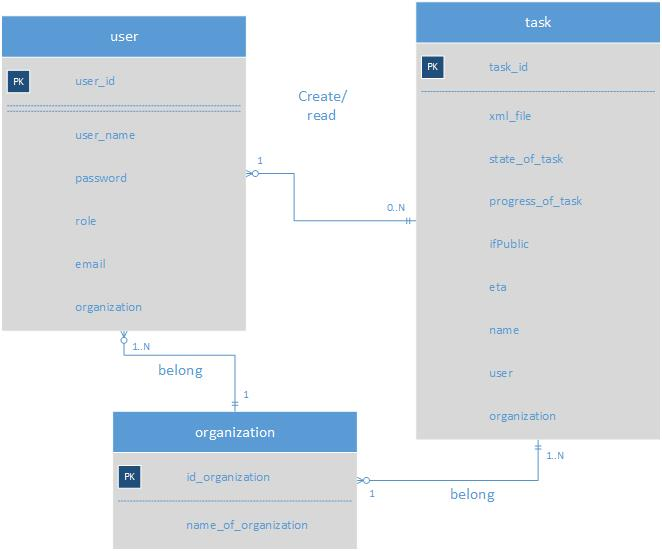
\includegraphics[scale=0.5]{ER.jpg} 
\caption{ER diagram}
\label{ER}

\end{center}

\end{figure}

Tento obrázok zobrazuje jednotlivé entity, ktoré sú potrebné na uloženie v databáze, každá z nich ma určité položky. ER diagrama sa skladá z 3 entít: user - entita, ktorá reprezentuje užívateľ, task - entita, ktorá reprezentuje úlohu a organization - entita, ktorá reprezentuje organizáciu. Výsledný návrh odpovedá skutočnosti, že každý užívateľ musí byť súčašťou organizácia, rovnako môže mať vytvorené 0 až N úloh. Taktiež pre zjednodušenie je každa úloha priradená priamo organizácií pre zlepšenie rýchlosti získania výsledkou a zjednodušenia ich nájdenia. Každá entita obsahuje primárny kľúč(jedná sa o silné entitné množiny), ktorý je odvodený od názvu a začína predponou \uv{id\_} a pokračuje názvom entity. Poďme sa pozrieť bližšie na jednotlivé entity. Entitná množina organization obsahuje 2 položky jednou z nich je primárny klúč a ďalšou názov organizácia podľa, ktorej sú zaraďovaný jednotlivý užívatelia. Ďalej prejdime k entitnej množine user. Táto entita má rovnako primárny kľúč. Ďalej obsahuje položku pre užívateľské meno(user\_name), heslo(password), email, užívateľskú rolu(role) a cudzí kľúcč organization, ktorý obsahuje na organizáciu. Nakoniec prejdime k entitnej množine task. Táto entitná množina obsahuje primárny kľúč, ďalej obsahuje xml súbor, ktorý reprezentuje danú úlohu(v našom prípade N dám), stav úloh(state\_of\_task, ktorý reprezentuje rôzne stavy úlohy), ktorý si podrobnejšie rozobereme. Úloha sa môže nachádzať v jednom z nasledujúcich stavov:
\begin{itemize}
\item NEW - úloha bola vytvorená
\item MODIFIED - xml súbor bol modifikovaný
\item WAITING - úloha čaká na spracovanie
\item IN\_PROGRESS - práve prebieha výpočet
\item PAUSED - úloha je pozastavená
\item COMPLETE - úloha je dokončená
\end{itemize}
Entitná množina task ďalej obsahuje položku, ktorá percentuálne hodnotí stav výpočtu úlohy(progress\_of\_task), čas do skončenia výpočtu úlohy(eta), nastavenie úlohy na privátnu alebo verejnú(ifPublic), názov úlohy(name) a cudzie kľúce user, ktorý odkazuje na užívateľa, ktorým bola úloha vytvorená a organization, ktorá odkazuje na organizáciu užívateľa, ktorým bola vytvorená. V ďalšej kapitole sa pozrieme na use case diagram.



\subsection{Diagram užitia}
Nasledujúci obrázok ukazuje príprady užitia systému:
\begin{figure}[htb]

\begin{center}

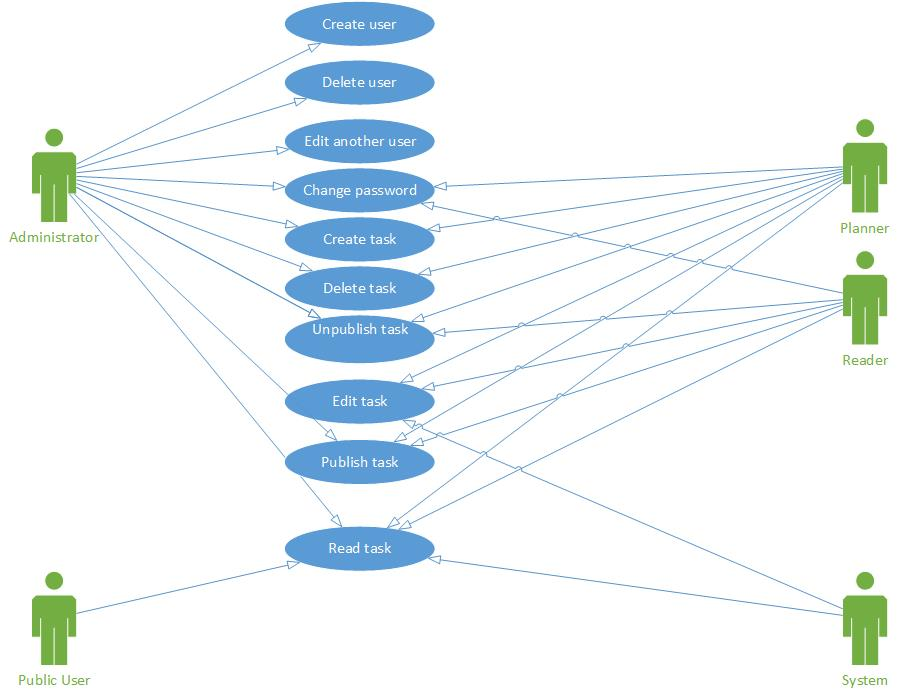
\includegraphics[scale=0.5]{UseCase.jpg} 
\caption{UseCase diagram}
\label{use}

\end{center}

\end{figure}
Na nasledujúcom obrázku č.\ref{use} môžme identifikovať 4 užívateľov systém. Public user je verejný úžívateľ, ktorý môže čítať úlohy, ktoré sú nastavené ako verejné(public). Systém môže načítať úlohy z databáze pre potreby výpočtu, z ktorými následne pracuje, a potom výsledky ukladá do databáze, teda edituje úlohy(tasky). Čitateľ(Reader) môže úlohy čítať, publikovať a odpublikovať. Plánovač môže úlohy čítať, vytvárať v databáze, mazať, editovať už vytvorené úlohy v rámci svojej organizácie,publikovať a odpublikovať úlohy a meniť vlastné heslo. Administrátor môže vytvárať úlohy, mazať úlohy , editovať úlohy, publikovať a odpublikovať úlohy. Rovnako si môže meniť heslo, vytvárať,mazať editovať organizácie a užívateľov.




\section{Návrh rozhrania}
Výsledné rozhranie kladie dôraz na jednoduchosť a prehľadnosť zobrazených úloh. Z tôhto dôvodu boli implementované mechanizmy vyhľadávanie úloh, organizácií a užívateľov. Rovnako možnosti lexikografického triedenia. Po prihlásení do systému Jednotlivé môžnosti sú následe zakompotované do záložiek, v ktorých je sprístupné príslušná funkčnosť. Výsledné rozhranie je prenositeľné aj na mobilné zaradenie, čo je spôsobené použitím frameworku Twitter Boostrap.


\section{Implementácie}
Aplikácie bola rozložená do viacerých tried podľa zodpovednosti daných komponent. Pri implementácií bolo použité JBoss Developer studo 7.1.1 GA spolu s JBoss AS 7.1.1 Final. Celý projekt boli založený na technológií maven, ktorú uľahčovala celý process vývoja a jeho následne nasadenie na JBoss server. Pre databázovú technológiu bol nainštalovaný mysql server nakonfigurovaný s príslunými prihlasovacími údajmi. Celý vývoj začal tvorbou balíka pre entitné triedy, ktoré pristupovali k databázami. Vývoj ďalej pokračoval tvorbou triedy, ktorá implementuje všetky potrebné operácie nad dátami. Následne treba správne nakonfigurovať datasource v JBoss AS, aby mohol správne pristupovať k databázmi vrátane prihlasovacích údajov. Následne pre správne priprájanie nasadeného maven projektu trebalo nastaviť súbor persistence.xml, do ktorého sa definovali entitné triedy a odkaz na datasource umiestneného na JBoss AS. Následne som sa sústredil na vývoj samotného užívatelského rozhrania. Užívateľské rozhranie som rozdelil do do 4 Managed bean, ktoré sa starajú o funkčnosť implementovaných xhtml stránok. Stránky sú celkom 4 , 3 pre užívatelské role, 4. pre prihlasovanie do systému. Každej stránke pritom odpovedá managed beana. Prihlasovacia stránka je upravená prostredníctvom Twitter Bootstrap-u, pričom obsahuje zabezpečenie prostredníctvom uživatelských rol. Rovnako obsahuje validáciu pred nekorektným prihlasovaním, ktoré môže byť spôsobené neznámym užívateľským meno alebo heslom. Následne je užívateľ presmerovaný na základe svojej role na príslušnú stránka. Každá stránka obsahuje záložky a podla svojej role dovodluje užívatelia vykonávať akcie. Základom každého zobrazenie je dátová tabulka h:datatable, ktorá zodpovedá príslušnému modelu(užívateľ, úloha, organizácia s príslušnými vlastnosťami), ktorá zobrazuje údaje na stránku a neustále obnovuje svoj obsah podľa obsahu v databázi. Príslušné riadky odpovedajú položkám v databázi pričom pre každú položku sa vzťahuje nejaká akcia, ktorá je reprezentovaná prislušným tlačidlom. Po stlačení tlačidla sa prislušna zmena prejaví na stránke rovnako ako aj na stránke. Vytváranie novej úlohy je reprezentované komponentov rich:upload, ktorá pochádza z frameworku Rich Faces. Táto komponenta zabezpečuje nahrávanie xml súborov, ktoré reprezentujú danú úlohu, celé je to zaobalené do formuláru, ktorý obsahuje položku na zadanie mena. Po stlačení tlačidla \uv{Create Task}, dôjde k zavolaniu methódy z managed beany príslušnej triedy, ktorá sa postará o vytvorenie úlohy v databázi a jej zobrazenie na stránke. V každú tabulku je možné zoraďovať podľa stĺpcov, deje sa to kliknutím na príslušný stĺpec, to spôsobí zavolanie metódy v managed bean-e, ktorá prejde všetky položky daného stĺpca, ktoré sú uložené v zozname a zoradí ich podľa stĺpcov. Obnovanie obsahuje sa realizuje prostredníctvom komponenty aj4:poll, ktorá je súčasťou frameworku Rich Faces. Táto komponenta neustála volá metódu, ktorá získava všetky položky z databáze, čím je zabezpečený aktuálny obsah tabuliek. Vyhľadávanie položiek v danej tabulke sa deje prostredníctvom formulára, do ktorého sa zadá vyhľadávaný reťazec a zvolí sa z vyskakovacie zoznamu, následna sa zavolá metóda, ktorá nastaví obsah h:datable na nájdené položky. Tento postup je rovnaký pre manažovanie organizácií a užívateĺov. Jednotlivé možnosti sú zakomponované od záložiek, ktoré sú implementované prostredníctvom twitter boostrap-u. Jednotlivé metódy sú pritom identické vo všetkých managed bean podľa užívatelskej role, až na to, že sú obmedzené podľa užívatelské role. Spustenie výpočtu sa deje prostredníctvom tlačidla \uv{Run Task}, to zavolé metódu \uv{Run Task} web service prostredníctvom http protokolu a predá mu ako parameter ID úlohy, ktorú má spustiť. Tá následne získa data z databáze a zaradí úlohu do fronty. Z fronty si odoberajú enterprise beany, ktoré sa môžu nachádzať kvôli rozprestrenie záťaže na viac serveroch. Tie si úlohu vyberú z actiemsq fronty a spustia výpočet. Priebežne pritom ukladajú údaje o stavu úlohy, času do ukončenia úlohy a percentuálnom ohodnotení úlohy. Po ukončení úlohy je uložené najlepšie možné riešenie do databáze. Užívateľ môže úlohy pozastaviť a to po stlačení tlačidla \uv{Stop Task}, ktoré zavolá metódu web service prostredníctvom protokolu http. Následne je možné úlohu opäť spustiť. Výsledky spracovania sú priebežne zobrazované(každé 2 sekundy) na užívateľské rozhranie. Rozhranie obsahuje validáciu, ktorá kontroluje všetky užívateľské vstupy.



\section{Testovanie}
Testovanie prebiehalo na servery JBoss AS 7.1.1 Final najprv prostredníctvom jednodúch JUnit testov, ktoré malo overiť komplikovanú fukčnosť metód. Následne sa pre overenie fukčnosti databáze použil framework Arqullian, ktorý umožňuje nasadenie tried priamo do Java EE kontajneru, čo zjednodušuje testovanie. Prostredníctvom tohto frameworku sa testovala celková fukčnosť aplikácie.

V ďalšej častie prebiehalo testovanie medzi konkrétnymi užívateľmi. Užívatelia testovali aplikáciu a hľadali buggy, ktoré neodhalilo predošlé testovanie.




\section{Vyhodnotenie aplikácie}
Po testovacej fáze nasledovala fáza vyhodnotenia aplikácie. Cielovým užívatelom bol poskytnutý prístup k aplikácií. Následne po vyskúšaní aplikácie vyplnili dotáznik, ktorá poskytoval celkový pohľad na aplikáciu.


















\chapter{Záver}



